\section{Experiments}


\subsection{Experimental Setup}

\paratitle{In-domain/Out-of-domain Tasks.}
We evaluate HaluAgent on both in-domain and out-of-domain datasets. As described in Section~\ref{sec: in-domain dataset}, we select HaluEval-QA, WebQA, Ape210K, HumanEval, and WordCnt as in-domain datasets. For out-of-domain datasets, we use a Chinese dataset, HalluQA~\cite{cheng2023evaluating}, and an English dataset, HaluEval 2.0~\cite{li2024dawn}, which cover diverse hallucination detection scenarios including knowledge, math, science texts. 
All datasets are associated with ground-truth response-level hallucination labels. We present the details in Appendix~\ref{app: ood_dataset}.

\paratitle{Sentence-level Tasks.}
HaluAgent performs fine-grained hallucination detection by segmenting sentences and provides sentence-level detection results. We use FacTool~\cite{chern2023factool} with annotated claim-level hallucination labels to evaluate the fine-grained detection capability. We consider each claim as a sentence and concatenate all claims as the input text. FacTool contains five sub-datasets: Chinese-QA, KB-QA, math problems, code generation, and scientific literature review. Since the code generation sub-dataset is collected from HumanEval and overlaps with our training data, we conduct sentence-level detection experiments on the other four sub-datasets. 

\paratitle{Baselines.}
Unlike previous work relied on powerful closed-source models like GPT-4, HaluAgent is built upon relatively smaller language model by performing fine-tuning on hallucination detection trajectory data.
Hence, we compare HaluAgent with two kinds of baselines: (1) Closed-source models: \emph{GPT-4 prompt} and \emph{GPT-4 pipeline} employ GPT-4 with simple task description prompts and our proposed detection pipeline, respectively; (2) Open-source models: \emph{Baichuan2-Chat (7B and 13B)}, which is the backbone model of HaluAgent. For other detection methods without comparison in this work, they are either implemented based on ChatGPT/GPT-4 (an unfair comparison) or focus solely on specific tasks, making it difficult to adapt to other tasks, as shown in Table~\ref{tab: detection-methods}.


\paratitle{Metrics.}
Hallucination detection is essentially a binary classification task. Consequently, we adopt \emph{Accuracy} and \emph{F1 score} as metrics for response-level detection evaluation. Considering the imbalanced hallucination data distribution at the sentence level, we adopt \emph{Accuracy}, \emph{Precision}, \emph{Recall}, and \emph{F1 score} for sentence-level detection.


\begin{table*}[htb]
\centering\small
\renewcommand{\arraystretch}{1.15}
\resizebox{\textwidth}{!}{
\begin{tabular}{@{}c@{\hspace{0.8\tabcolsep}}lcc|cc|cc@{}}
\toprule
\multicolumn{1}{c}{\multirow{2}{*}{Types}} & \multicolumn{1}{l}{\multirow{2}{*}{Datasets}} & \multicolumn{2}{c}{GPT-4} & \multicolumn{2}{c}{Baichuan2-Chat} & \multicolumn{2}{c}{HaluAgent} \\ \cmidrule(l){3-4} \cmidrule(l){5-6} \cmidrule(l){7-8} 
\multicolumn{1}{l}{} & \multicolumn{1}{c}{} & prompt & \multicolumn{1}{c}{pipeline} & 7B & 13B & 7B & 13B  \\ \midrule
\multirow{6}{*}{\begin{tabular}[c]{@{}c@{}}{In-domain}\\ {Datasets}\end{tabular}} & {WebQA} & 82.00/35.71 & \underline{91.00}/\underline{57.14} & 51.00/14.04 & 54.00/\textbf{61.67} & 80.00/54.55 & \textbf{82.83}/51.43  \\
 & {Ape210K} &72.33/74.21 & \underline{76.63}/\underline{75.10} & 49.00/7.27 & 51.33/58.29& 72.00/72.55& \textbf{73.40}/\textbf{73.68}  \\
 & {HumanEval} & 71.43/79.07& \underline{93.44}/\underline{94.12} & 34.92/49.38& 47.62/19.51 & \textbf{93.44}/\textbf{94.12} & \textbf{93.44}/\textbf{94.12} \\
 & {WordCnt} & 56.00/66.15 & \underline{100.00}/\underline{100.00} & 43.00/16.00 & 46.00/59.70 & \textbf{100.00}/\textbf{100.00} & \textbf{100.00}/\textbf{100.00} \\
 & {HaluEval-QA} & 62.00/42.42 & \underline{77.53}/\underline{75.61} & 53.19/46.34 & 60.00/67.74 & 67.00/67.33 & \textbf{71.00}/\textbf{72.38} \\\cmidrule{2-8}
 & {Overall} & 69.76/71.66 & \underline{85.10}/\underline{83.12} & 46.44/32.20 & 52.70/55.58 & 79.70/79.50 & \textbf{81.86}/\textbf{80.69} \\ \midrule
\multirow{3}{*}{\begin{tabular}[c]{@{}c@{}}{Out-of-domain}\\ {Datasets}\end{tabular}} & {HalluQA} & 61.00/74.84 & \underline{85.11}/\underline{89.23} &33.00/12.99 & 56.00/67.16 & 67.48/76.09 & \textbf{78.16}/\textbf{83.75}  \\
 & {HaluEval 2.0} & 63.00/74.13 & \underline{85.71}/\underline{87.36} & 54.00/69.33 & 43.00/46.73 & 75.00/76.19 & \textbf{79.00}/\textbf{78.79}  \\ \cmidrule{2-8}
 & {Overall} & 62.00/74.50& \underline{85.25}/\underline{88.76} & 43.50/50.22 & 49.50/58.10 & 69.97/76.12 & \textbf{78.43}/\textbf{82.45}   \\ 
 \bottomrule
\end{tabular}
}
\caption{Evaluation results at Accuracy and F1 score on in-domain and out-of-domain datasets. \textbf{Bold} denotes the best methods among open-source models; \underline{underline} denotes the best methods among closed-source models.}
% \vspace{-0.2cm}
\label{tab: main-results}
\end{table*}


\begin{table*}[htb]
\centering\small
\renewcommand{\arraystretch}{1.15}
\resizebox{\textwidth}{!}{
\begin{tabular}{lcccc}
\toprule
 Models & Chinese-QA & KB-QA & Math & Science \\
 \midrule
 GPT4-prompt & 54.93/59.40/33.17/42.57 & 75.97/39.29/50.00/44.00 & 55.27/49.25/23.74/32.04 & 59.14/64.71/81.82/72.26\\
 GPT4-pipeline &79.76/64.71/50.00/56.41 & 84.12/85.31/93.21/89.09 & 91.61/79.66/78.33/78.99 & 95.72/96.77/98.04/97.40\\
 Baichuan2-Chat 7B  & 65.15/15.02/29.17/19.83 & 49.77/38.78/19.59/26.03  & 68.07/17.91/21.43/19.51 & 24.19/9.80/83.33/17.54\\
 Baichuan2-Chat 13B & 56.82/21.70/22.67/22.17 & 65.41/30.77/30.00/30.38 & 70.97/13.85/20.93/16.67  & 18.82/1.31/100.00/2.58\\
 HaluAgent-7B  & 73.57/32.96/55.97/41.49  & 83.33/41.82/82.14/55.42 & 85.39/81.13/59.72/68.80 & 90.27/94.77/93.55/94.16\\
 HaluAgent-13B & 75.47/33.80/56.25/42.23 & 81.97/62.07/85.71/72.00 & 87.50/64.52/72.73/68.38 & 92.39/96.05/94.81/95.42\\
\bottomrule
\end{tabular}
}
\caption{Evaluation results of sentence-level detection on the four subsets of FacTool.}
\label{tab: sentence-level results}
\vspace{-0.2cm}
\end{table*}

\subsection{Response-level Detection}

We present the evaluation results on in-domain and out-of-domain datasets in Table~\ref{tab: main-results}.

First, by comparing GPT-4 and Baichuan2-Chat, we can observe a large performance gap between closed-source and open-source models when detecting hallucinations solely based on their internal knowledge. In Table~\ref{tab: main-results}, 
GPT-4 achieves detection accuracies of 82.00\% and 72.33\% on WebQA and Ape210K respectively, whereas Baichuan2-Chat only achieves 51.00\% and 49.00\%. 
This underscores the considerable difference in hallucination detection capabilities between these models.

Second, implementing a fine-grained detection framework and incorporating extensive tools can enhance the hallucination detection performance of LLMs across various tasks. Compared to GPT-4 prompt, GPT-4 pipeline consistently yields better detection results across all datasets. 
Especially for tasks that require tools to detect the hallucinations such as WordCnt, our tool-assistant framework boosts the detection accuracy of GPT-4 from 56.00\% to 100.00\%. This demonstrates that guiding the model to utilize appropriate tools tailored to the specific text is an effective strategy to enhance hallucination detection capabilities.

Finally, based on trajectory fine-tuning, smaller open-source models can be effective autonomous agents for hallucination detection, narrowing the gap with closed-source models. As can be observed from Table~\ref{tab: main-results}, HaluAgent consistently improves detection performance across in-domain datasets compared to Baichuan2-Chat. 
For instance, on the WebQA dataset, HaluAgent 7B and 13B improve the detection accuracy from 51.00\%, 60.00\% to 80.00\%, 71.00\%, respectively.
Furthermore, substantial performance improvements are observed on out-of-domain datasets, with accuracy increasing from 33.00\% to 67.48\% (7B) for HalluQA and from 43.00\% to 79.00\% (13B) for HaluEval 2.0.  
With tool utilization and agent capabilities, HaluAgent achieves performance comparable to or even higher than GPT-4 prompt across all tasks, showing strong generalization capability.



\subsection{Sentence-level Detection}

In our framework, HaluAgent is capable of detecting hallucinations for each individual sentence. Thus, we evaluate the accuracy of HaluAgent in identifying hallucinations at the sentence level. 

The sentence-level detection results are shown in Table~\ref{tab: sentence-level results}. As we can see, HaluAgent achieves much higher F1 score compared to Baichuan2-Chat, especially for those tasks where the detection results can be precisely judged via tools. For example, HaluAgent 13B achieves an accuracy of 87.50\% on the math dataset, and F1 score of 95.42\% on the scientific literature review dataset, approaching the performance of the GPT-4 pipeline. We attribute this improvement to the fine-grained design of the HaluAgent framework and its capability to store and reflect on detection results for each sentence.


\begin{figure}[tb]
	\centering
	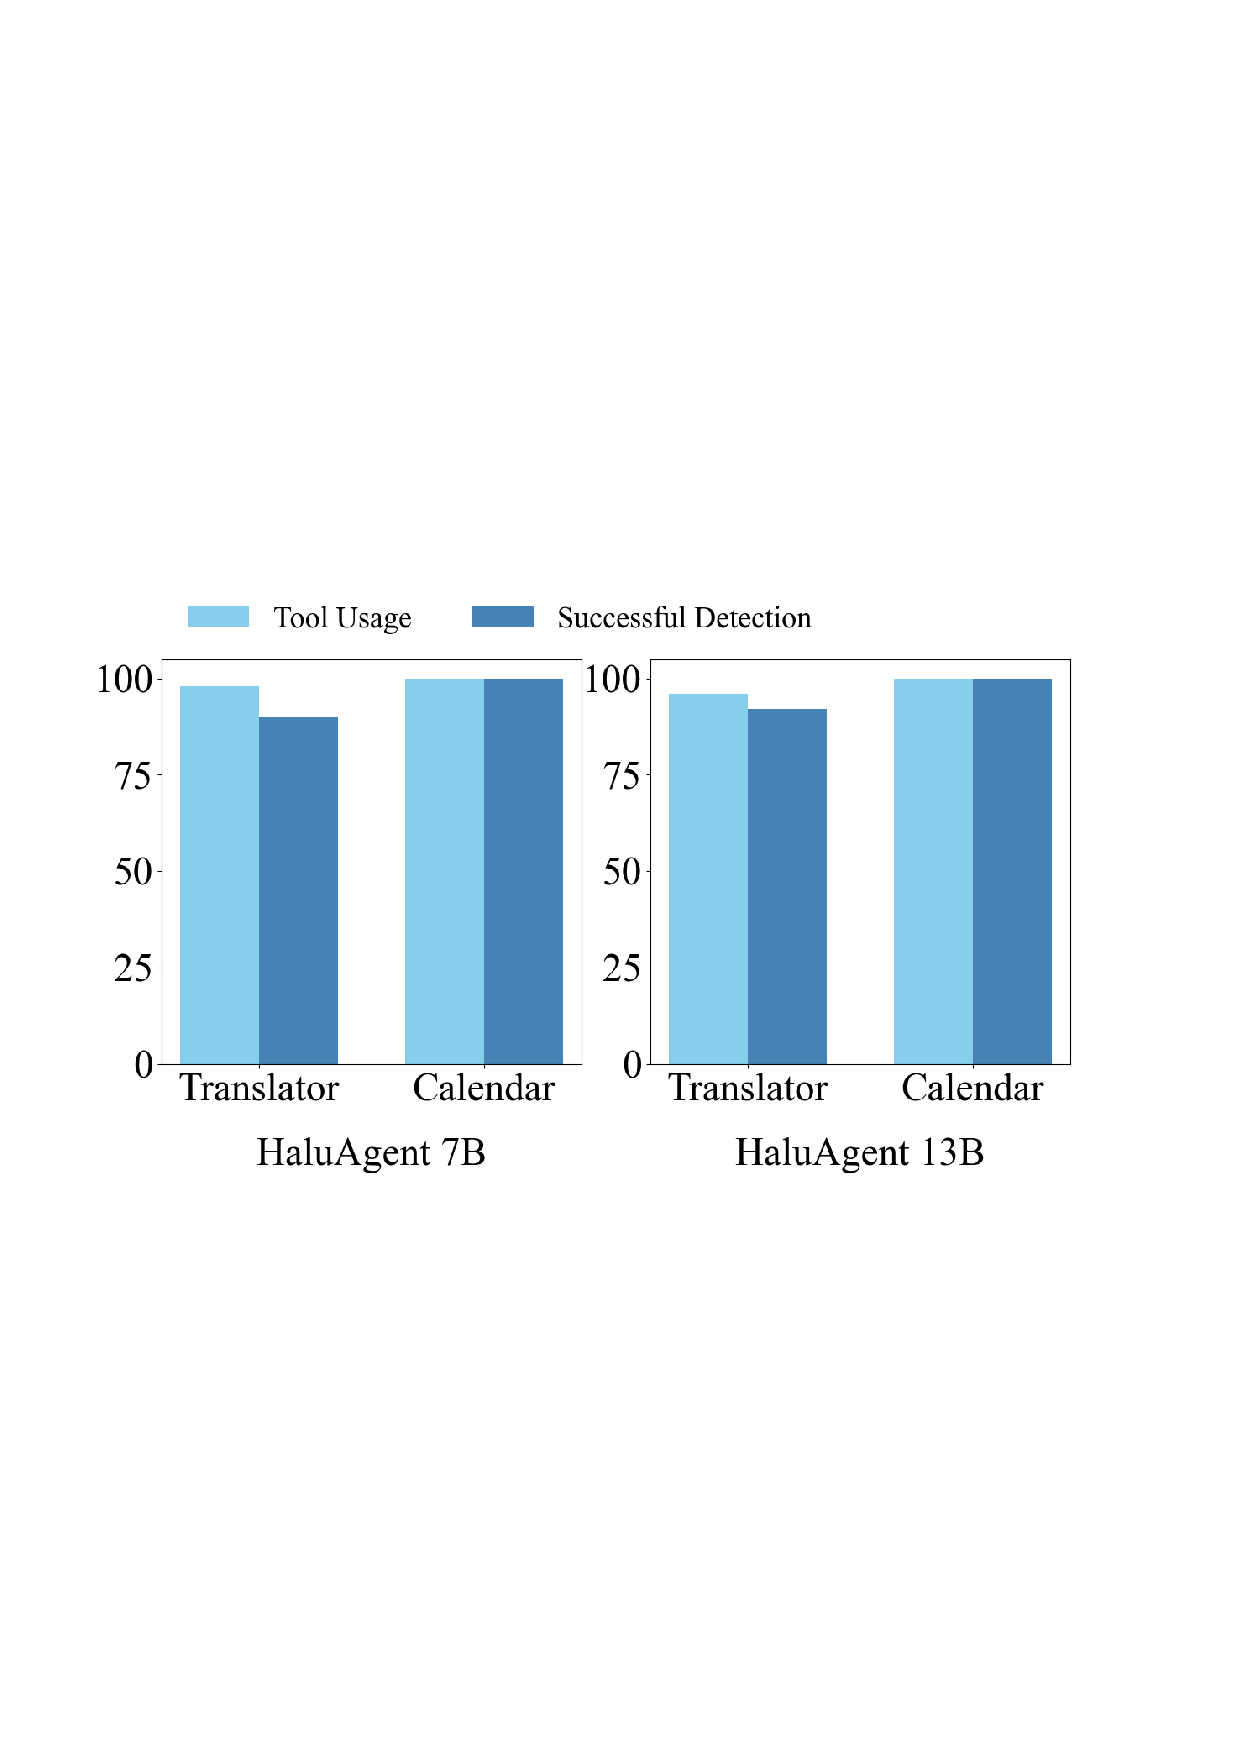
\includegraphics[width=0.48\textwidth]{image/new_tool.pdf}
	\caption{The usage rate of new tools and the proportion of successful detection.}
	\label{fig: new_tool}
	\vspace{-0.2cm}
\end{figure}

\begin{figure*}[tb]
	\centering
        \small
	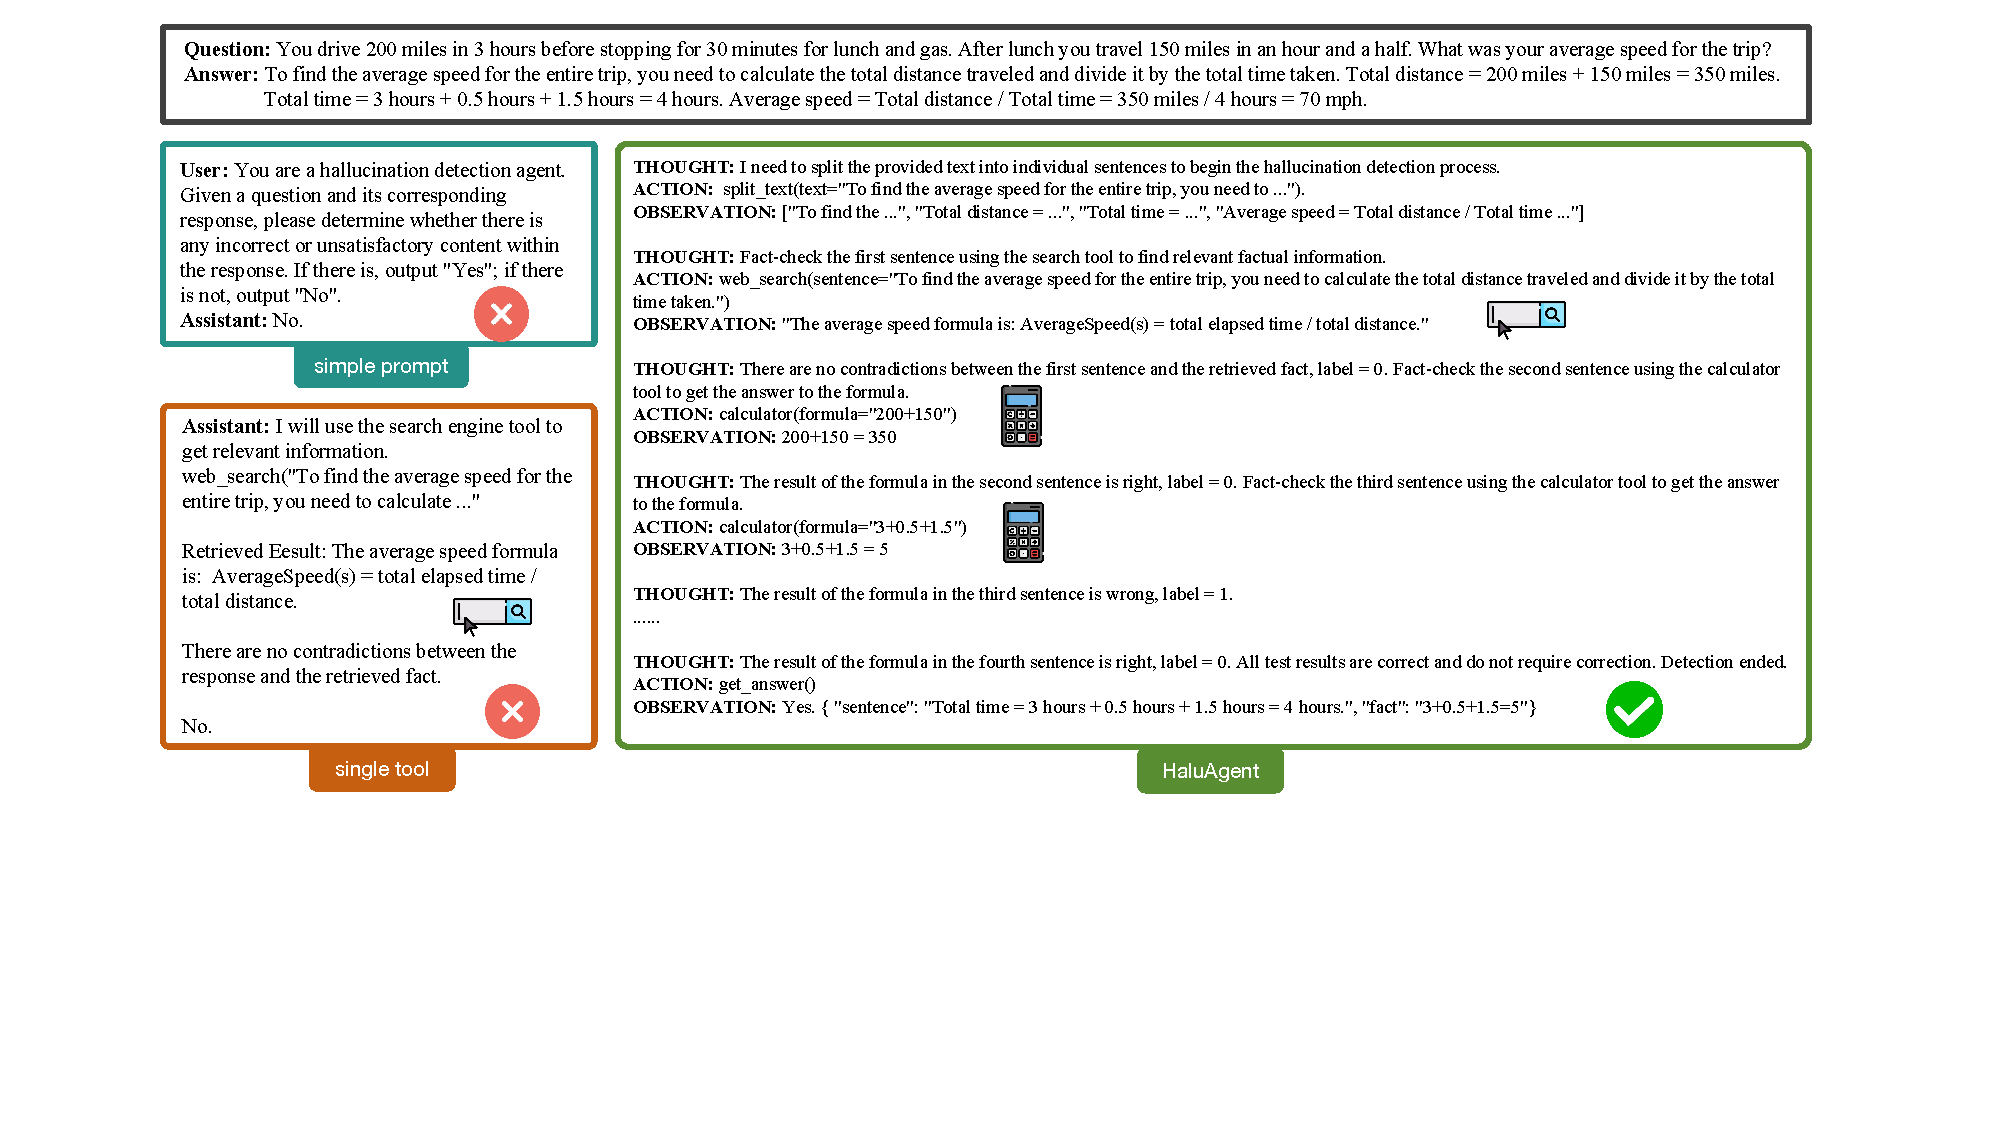
\includegraphics[width=1.00\textwidth]{image/casestudy.pdf}
	\caption{Case study between GPT-4 with a simple prompt and single tool, and the HaluAgent framework.}
	\label{fig: case study}
	\vspace{-0.2cm}
\end{figure*}

\subsection{Further Analysis}

% \subsubsection{Ablation Study}

\paratitle{Extensibility Study.}
To verify the extensibility of our HaluAgent framework, we introduce new tools to the fine-tuned models and test their abilities to use these tools for hallucination detection. Specifically, we incorporate a translator and a calendar tool into the HaluAgent toolbox for handling texts related to translation and date calculations. We provide instructions and two examples as in-context demonstrations to guide the model to use these new tools.
For evaluation, we employ ChatGPT to generate 100 samples involving translation and date calculation. Instruction and dataset details can be found in Appendix~\ref{app: scalability_exp}.

We measure the proportion of correct tool usage and successful task completion rate by HaluAgent in Figure~\ref{fig: new_tool}. As we can see, HaluAgent 7B and 13B achieve a usage rate of over 95\% for the translator tool, and the usage rate for the calendar tool is 100\%. Due to the models' inherent multilingual capabilities, they sometimes directly assess the accuracy of the translation result instead of invoking the translator tool. With the assistance of the appropriate tools, HaluAgent achieves a success rate of 100\% in hallucination detection for date calculation and over 90\% success rate for translation task. These experimental results indicate that with instructions and demonstrations, HaluAgent can effectively use new tools to complete hallucination detection tasks without additional fine-tuning. 

\paratitle{Case Study.}
To qualitatively demonstrate the effectiveness of HaluAgent, we present a case study about average speed calculation, which involves both commonsense knowledge and mathematical calculations. 
We compare HaluAgent with two hallucination detection methods based on GPT-4 with simple prompts and search engine tool, as shown in Figure~\ref{fig: case study}. 
As we can see, GPT-4 fails to detect the minor calculation errors (\ie \textit{3 hours + 0.5 hours + 1.5 hours = 4 hours}) when only provided with a simple prompt of task description. 
Meanwhile, GPT-4 with a search engine tool can only verify the formula for average speed in the response but cannot check the correctness of each calculation step. Consequently, both methods yield incorrect detection results.
In contrast, HaluAgent autonomously plans and selects suitable tools for different parts of the text (\ie search engine for knowledge checks and calculator for calculation checks), allowing for accurate verification of the content. This highlights HaluAgent's capability to effectively verify complex texts with mixed types of hallucinations.
